% Unit 3.5-4: Momentum Flow (continued), Energy, Work & Energy, Conservative Forces
% Pages 66–92

\chapter{Momentum Flow and Pressure}

\section{Momentum Flux Density}

If the surface is \emph{not} perpendicular to the flow, the momentum rate is
\[
    \dot{P} = \rho_m v^2 A \cos\theta.
\]

\begin{definition}[Flux Density of the Stream]
The momentum flux density $\vect{J}$ of a stream is
\[
    \vect{J} = \rho_m v^2 \,\uvect{v}.
\]
\end{definition}

If one lets $\vect{A}$ be a vector perpendicular to the surface with magnitude equal to the area, then
\[
    \dot{\vect{P}} = (\vect{J} \cdot \vect{A})\,\uvect{v}.
\]

\begin{itemize}
    \item Flux is \textbf{positive} when $\vect{J} \cdot \vect{A} > 0$; flux is \textbf{negative} when $\vect{J} \cdot \vect{A} < 0$.
    \item The total force on a system due to a number of sources of momentum flow is
    \[
        F_{\text{tot}} = \sum_k \dot{P}_k = \sum_k (\vect{J} \cdot \vect{A}_k)\,\uvect{v}_k.
    \]
    \item As the number of elements increases, this sum becomes a \textbf{surface integral}.
\end{itemize}

A more helpful way to calculate the force on a system with several sources of momentum flow is
\begin{formula}[Total Force from Momentum Flow]
\[
    F_{\text{tot}} = \dot{P}_{\text{in}} - \dot{P}_{\text{out}}.
\]
\end{formula}

\begin{example}[Pressure of a Gas]
Consider a box of $n$ particles each with mass $m$.

\begin{figure}[H]
    \centering
    \caption{Box of gas particles; surface $A$ on one face.}
\end{figure}

We want to find the momentum transport through a surface $A$.

At any moment the density of particles moving \emph{toward} the wall is $\rho/2$, so
\[
    \dot{P}_x = \frac{\rho}{2}\,v_x^2\,A.
\]
The $v_x$ here is the $x$-component of velocity.

Momentum flow \emph{away} from the wall:
\[
    \dot{P}_{-x} = \frac{\rho}{2}\,v_x^2\,A.
\]
Thus
\[
    F_x = \dot{P}_x - \dot{P}_{-x} = \rho v^2 A.
\]

For arbitrary velocities (using averages):
\[
    \widetilde{F}_x = \dot{P}_x - \dot{P}_{-x} = \rho\,\overline{v_x^2}\,A.
\]

The pressure is
\[
    \mathcal{P} = \frac{F}{A} = \rho\,\overline{v_x^2}.
\]

Since $\overline{v^2} = \overline{v_x^2} + \overline{v_y^2} + \overline{v_z^2}$ and by isotropy each component is equal,
\begin{formula}[Gas Pressure]
\[
    \boxed{\mathcal{P} = \frac{1}{3}\,\rho\,\overline{v^2}.}
\]
\end{formula}
\end{example}

\begin{example}[Pressure on a Dike]
A curved dike deflects a stream of fluid through an angle $\Delta\theta$. Let the incoming momentum flux be
\[
    \dot{P}_{\text{in}} = \rho v^2 A \,\uvect{v}_c, \qquad \dot{P}_{\text{out}} = \rho v^2 A\,\uvect{v}_d.
\]
So
\[
    \dot{P} = \rho v^2 A\,(\uvect{v}_c - \uvect{v}_d) = \rho v^2 A \bigl(2\sin(\Delta\theta/2)\bigr).
\]
The force per unit area (pressure) on the dike element of length $R\,\Delta\theta$ and height $h$ is
\[
    \mathcal{P} \approx \frac{\dot{P}}{R\,\Delta\theta \cdot h} = \frac{\rho v^2 A\,\Delta\theta}{R\,\Delta\theta\, h} = \frac{\rho v^2 A}{R\,h} = \frac{\rho v^2 w}{R},
\]
where $w = A/h$ is the width.
\end{example}

\chapter{Energy}

\section{Work–Energy Theorem in One Dimension}

Force is often known as a function of \emph{position}, not time. Many problems take the form
\[
    m\,\dv{v}{t} = F(x).
\]
To solve, integrate both sides with respect to $x$:
\[
    m \int_{x_a}^{x_b} \dv{v}{t}\,dx = \int_{x_a}^{x_b} F(x)\,dx.
\]
Replace $dx$:
\[
    dx = \left(\dv{x}{t}\right)dt = v\,dt,
\]
so
\begin{align*}
    m\int_{x_a}^{x_b}\dv{v}{t}\,dx &= m\int_{t_a}^{t_b} \dv{v}{t}\,v\,dt \\
    &= m\int_{t_a}^{t_b} \dv{}{t}\!\left(\tfrac{1}{2}v^2\right)dt \\
    &= \tfrac{1}{2}mv^2\Big|_{t_a}^{t_b}.
\end{align*}

\begin{formula}[Work–Energy Theorem (1D)]
\[
    \boxed{\tfrac{1}{2}mv_b^2 - \tfrac{1}{2}mv_a^2 = \int_{x_a}^{x_b} F(x)\,dx.}
\]
\end{formula}

\subsection{Derivation of GPE near Earth's Surface}

\[
    \tfrac{1}{2}mv_b^2 - \tfrac{1}{2}mv_a^2 = -mg\int_{x_a}^{x_b} dx = -mg(x_b - x_a).
\]
Letting $v_a = v_b = 0$ gives $\tfrac{1}{2}mv_a^2 = mgh$.

\subsection{Derivation of Spring Potential Energy}

\begin{figure}[H]
\begin{center}
\begin{tikzpicture}[scale=0.9, >=Stealth]
  % Wall
  \fill[pattern=north east lines] (-0.2,-0.35) rectangle (0,0.35);
  \draw[thick] (0,-0.35) -- (0,0.35);
  % Spring
  \draw[thick, decorate, decoration={zigzag, segment length=5pt, amplitude=3pt}]
    (0,0) -- (2.8,0);
  % Mass
  \fill[gray!40] (2.8,-0.3) rectangle (3.4,0.3);
  \draw[thick] (2.8,-0.3) rectangle (3.4,0.3);
  \node at (3.1,0) {$M$};
  % Displacement arrow
  \draw[<->,blue] (0,-0.6) -- (3.1,-0.6) node[midway,below]{$x_0$};
  % Equilibrium dashed line
  \draw[dashed,gray] (1.8,-0.5) -- (1.8,0.5) node[above,scale=0.8]{equil.};
\end{tikzpicture}
\end{center}
\caption{Mass on a spring; equilibrium at $x=0$, initial displacement $x_0$ from equilibrium.}
\label{fig:spring_pe}
\end{figure}

With $F = -kx$:
\[
    \tfrac{1}{2}Mv^2 - \tfrac{1}{2}Mv_0^2 = -k\int_{x_0}^{x} x\,dx = -\tfrac{1}{2}kx^2 + \tfrac{1}{2}kx_0^2,
\]
thus
\[
    v^2 = \frac{k}{M}(x_0^2 - x^2).
\]
Separating variables:
\[
    \frac{1}{\sqrt{x_0^2 - x^2}}\,dx = \sqrt{\frac{k}{M}}\,dt,
\]
\[
    \sin^{-1}\!\left(\frac{x}{x_0}\right) - \sin^{-1}(1) = \omega t,
\]
\begin{formula}[SHO Solution from Energy]
\[
    \boxed{x = x_0 \sin\!\left(\omega t + \tfrac{\pi}{2}\right) = x_0\cos(\omega t).}
\]
\end{formula}

\section{Work and Energy}

\begin{definition}[Kinetic Energy]
\[
    K_a \defeq \tfrac{1}{2}Mv_a^2.
\]
\end{definition}

\begin{definition}[Work]
\[
    W_{ba} \defeq \int_{x_a}^{x_b} F\,dx = K_b - K_a \quad \text{(Work–Energy Theorem)}.
\]
\end{definition}

Units of energy: Joule, $\mathrm{J} = \frac{\mathrm{kg}\cdot\mathrm{m}^2}{\mathrm{s}^2} = \frac{M \cdot L^2}{T^2}$.

\section{Integrating Motion in Several Directions}

Let $\vect{r}$ be a position vector. We need to solve
\[
    \vect{F}(\vect{r}) = m\dv{\vect{v}}{t}.
\]
Dot both sides with $\Delta\vect{r}$:
\[
    \vect{F} \cdot \Delta\vect{r} = m\dv{\vect{v}}{t} \cdot \Delta\vect{r} = F\,\Delta r\cos\theta = m\dv{\vect{v}}{t}\cdot\Delta\vect{r}.
\]

Since $\Delta\vect{r} = \vect{v}\,\Delta t$ (reason why energy is path-independent!):
\[
    m\dv{\vect{v}}{t}\cdot\Delta\vect{r} = m\dv{\vect{v}}{t}\cdot\vect{v}\,\Delta t = m\,\frac{1}{2}\dv{}{t}(v^2)\,\Delta t.
\]
Thus
\[
    \vect{F}\cdot\Delta\vect{r} = \frac{m}{2}\dv{}{t}(v^2)\,\Delta t.
\]

Next, divide the trajectory from $\vect{r}_a$ to $\vect{r}_b$ into short segments:

\begin{figure}[H]
    \centering
    \caption{Trajectory divided into short segments $\Delta\vect{r}_j$ at positions $\vect{r}_j$.}
\end{figure}

Thus $\vect{F}(\vect{r}_j)\cdot\Delta\vect{r}_j = \dfrac{m}{2}\dv{}{t}(v_j^2)\,\Delta t_j$.

Summing:
\[
    \sum_{j=1}^{N} \vect{F}(\vect{r}_j)\cdot\Delta\vect{r}_j = \sum_{j=1}^{N} \frac{m}{2}\dv{}{t}(v_j^2)\,\Delta t_j.
\]
In the limit:
\[
    \int_{\vect{r}_a}^{\vect{r}_b} \vect{F}(\vect{r})\cdot d\vect{r} = \frac{m}{2}\int_{t_a}^{t_b}\dv{}{t}(v^2)\,dt = \frac{m}{2}\,v^2\Big|_{t_a}^{t_b} = \tfrac{1}{2}mv_b^2 - \tfrac{1}{2}mv_a^2.
\]

\begin{formula}[Work–Energy Theorem (3D)]
\[
    \boxed{\int_{\vect{r}_a}^{\vect{r}_b} \vect{F}\cdot d\vect{r} = \tfrac{1}{2}mv_b^2 - \tfrac{1}{2}mv_a^2.}
\]
\end{formula}

\begin{example}[General Escape Velocity]
The gravitational force on a mass $m$ due to a planet of mass $M_e$ is
\[
    \vect{F} = -\frac{GM_e m}{r^2}\,\uvect{r} = -mg\frac{R_e^2}{r^2}\,\uvect{r}.
\]
In spherical coordinates, $d\vect{r} = dr\,\uvect{r} + r\,d\theta\,\tthat$, so
\[
    \vect{F}\cdot d\vect{r} = -mg\frac{R_e^2}{r^2}\,dr \quad (\text{since } \uvect{r}\cdot\tthat = 0).
\]
Thus
\[
    \tfrac{1}{2}mv_f^2 - \tfrac{1}{2}mv_0^2 = -mgR_e^2\int_{R_e}^{r}\frac{dr}{r^2} = -mgR_e^2\left(\frac{1}{r} - \frac{1}{R_e}\right).
\]
As $r\to\infty$:
\begin{formula}[Escape Velocity]
\[
    v_{\text{esc}} = \sqrt{2g R_e}.
\]
\end{formula}
\end{example}

\section{Applying the Work–Energy Theorem}

Because $W_{ba} = \int_a^b \vect{F}\cdot d\vect{r}$ for non-conservative forces, $\vect{F}$ and the actual path must be known.

\begin{itemize}
    \item Most forces are conservative, however.
    \item When motion is \emph{constrained}, the constraint force does no work (the force integral only depends on tangential forces).
\end{itemize}

\begin{definition}[Work (general)]
\[
    \int_C \vect{F}\cdot d\vect{r} = W.
\]
\end{definition}

\begin{definition}[Power]
\[
    \dv{W}{t} = \vect{F}\cdot\vect{v}.
\]
\end{definition}

\section{Conservation of Energy}

\begin{formula}[Conservation of Energy]
\[
    W = \int_{\vect{r}_a}^{\vect{r}_b} \vect{F}\cdot d\vect{r} = -U(\vect{r}_b) + U(\vect{r}_a) = K_b - K_a,
\]
\[
    \Rightarrow\quad K_a + U(\vect{r}_a) = K_b + U(\vect{r}_b) \quad \text{(total energy is conserved)}.
\]
\end{formula}

For a closed path, $W = \oint_C \vect{F}\cdot d\vect{r} = U(\vect{r}_a) - U(\vect{r}_a) = 0$.

Thus:
\[
    U = -\oint \vect{F}\cdot d\vect{r}, \qquad \vect{F} = -\grad U, \qquad F = -\dv{U}{r}.
\]

\section{Energy Diagrams}

\begin{figure}[H]
\begin{center}
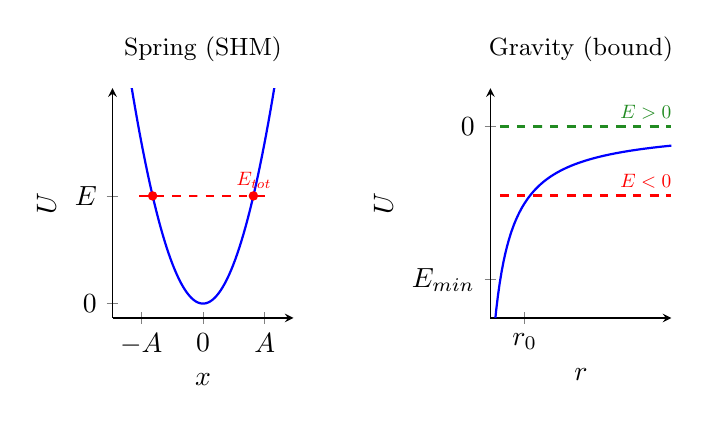
\begin{tikzpicture}
  %--- Left: SHM parabola ---
  \begin{scope}
  \begin{axis}[
    name=ax1,
    width=0.32\textwidth, height=4.5cm,
    xlabel={$x$}, ylabel={$U$},
    title={\small Spring (SHM)},
    xmin=-2.2,xmax=2.2, ymin=-0.2, ymax=3,
    xtick={-1.5,0,1.5}, xticklabels={$-A$,$0$,$A$},
    ytick={0,1.5}, yticklabels={$0$,$E$},
    axis lines=left, samples=80,
  ]
    \addplot[thick,blue,domain=-2:2]{x^2};
    \addplot[thick,dashed,red,domain=-1.55:1.55]{1.5} node[pos=0.9,above,scale=0.7]{$E_\text{tot}$};
    \addplot[only marks,mark=*,mark size=1.5pt,red] coordinates {(-1.225,1.5)(1.225,1.5)};
  \end{axis}
  \end{scope}
  %--- Center: gravitational potential well ---
  \begin{scope}[xshift=4.8cm]
  \begin{axis}[
    name=ax2,
    width=0.32\textwidth, height=4.5cm,
    xlabel={$r$}, ylabel={$U$},
    title={\small Gravity (bound)},
    xmin=0.3, xmax=4, ymin=-2.5, ymax=0.5,
    xtick={1}, xticklabels={$r_0$},
    ytick={-2,0}, yticklabels={$E_\text{min}$,$0$},
    axis lines=left, samples=100,
  ]
    \addplot[thick,blue,domain=0.38:4]{-1/x};
    \addplot[thick,dashed,red,domain=0.5:4]{-0.9} node[pos=0.85,above,scale=0.7]{$E<0$};
    \addplot[thick,dashed,ForestGreen,domain=0.5:4]{0.0} node[pos=0.85,above,scale=0.7]{$E>0$};
  \end{axis}
  \end{scope}
\end{tikzpicture}
\end{center}
\caption{Energy diagrams. \textit{Left}: Spring force — parabolic $U(x) = kx^2/2$; $E_{\text{tot}}$ is a horizontal red dashed line and the amplitude (turning points) is where $KE=0$. \textit{Right}: Gravitational $U(r) = -GMm/r$; bound orbit has $E<0$ (red dashed), unbound orbit has $E>0$ (green dashed).}
\label{fig:energy_diagrams}
\end{figure}

Non-conservative forces: $\oint \vect{F}\cdot d\vect{r} \neq 0$ (depends on path taken). Example: friction.

Thus,
\[
    E_{\text{tot}} = U + K + W_{\text{non-cons.}} = U + K + \int_{\vect{a}}^{\vect{b}} \vect{F}_f \cdot d\vect{r}.
\]

\begin{example}[Block on an Incline]
\begin{figure}[H]
    \centering
    \caption{Block sliding down an incline of angle $\theta$ and height $h$, path length $s = h/\sin\theta$.}
\end{figure}

\begin{itemize}
    \item Start: $U_a = mgh$, $K_a = 0$, $E_a = U_a + K_a = mgh$.
    \item End: $U_b = 0$, $K_b = \tfrac{1}{2}mv_b^2$, $E_b = \tfrac{1}{2}v_b^2$.
    \item Work by friction:
    \[
        W_f = \int_a^b \vect{F}_{fr}\cdot d\vect{r} = -\int_a^b \mu F_N\,ds = -\mu mg\cos\theta \cdot s = -\mu mg\cos\theta \cdot \frac{h}{\sin\theta}.
    \]
\end{itemize}
\end{example}

\chapter{Additional Energy Examples}

\section{Minimum Height for Ball to Go Around a Loop}

\begin{figure}[H]
\begin{center}
\begin{tikzpicture}[scale=0.85, >=Stealth]
  % Ground level
  \draw[thick] (0,0) -- (7.5,0);
  % Ramp (inclined)
  \draw[thick] (0,3.0) -- (2.2,0);
  % Height label
  \draw[<->,gray] (-0.3,0) -- (-0.3,3.0) node[midway,left]{$h$};
  % Ball on ramp
  \fill[blue!60] (0.9,1.5) circle[radius=0.13];
  % Loop circle
  \draw[thick] (5.0,1.0) circle[radius=1.0];
  % Center of loop
  \fill (5.0,1.0) circle[radius=0.04];
  % Radius label
  \draw[<->,gray] (5.0,1.0) -- (5.0,2.0) node[midway,right]{$R$};
  % Ball at top of loop
  \fill[blue!60] (5.0,2.0) circle[radius=0.13];
  % Force arrow at top
  \draw[->,red] (5.0,2.0) -- (5.0,1.4) node[right,scale=0.8]{$mg+N$};
  % Height 2R label
  \draw[<->,gray] (4.1,0) -- (4.1,2.0) node[midway,left]{$2R$};
  % Ball at bottom
  \fill[blue!60] (4.0,0) circle[radius=0.13];
\end{tikzpicture}
\end{center}
\caption{Ball released from height $h$ slides down a frictionless ramp and around a loop of radius $R$. At the top of the loop (height $2R$) the centripetal condition requires $N + mg = mv_t^2/R$.}
\label{fig:loop_the_loop}
\end{figure}

Total energy: $mgh$.

At the bottom of the loop: $\tfrac{1}{2}mv^2 = mgh \Rightarrow v = \sqrt{2gh}$.

We want the ball to make it all the way around without falling at the top.

At the top of the loop (height $2R$), the centripetal force equation is:
\[
    mg + N = m\frac{v_t^2}{R}.
\]
We want $N \geq 0$, so
\[
    \frac{mv_t^2}{R} \geq mg.
\]
By energy conservation from start to top:
\[
    mg(h - 2R) = \tfrac{1}{2}mv_t^2 \Rightarrow v_t^2 = 2g(h-2R).
\]
Substituting into the constraint:
\[
    \frac{m \cdot 2g(h-2R)}{R} - mg \geq 0,
\]
\[
    \frac{m\,g(h-2R)}{R} \cdot 2 \geq mg,
\]
\[
    2h - 4R \geq R, \qquad 2h \geq 5R,
\]
\begin{formula}[Minimum Height for Loop]
\[
    \boxed{h > \frac{5}{2}R.}
\]
\end{formula}

\subsection{Higgs Potential}

\begin{itemize}
    \item A particle that originally gives other particles mass.
    \item Discovered at CERN LHC.
    \item Smashes particles together to discover their properties.
\end{itemize}

\section{Integrating \texorpdfstring{$\vect{F}\cdot d\vect{r}$}{F dot dr}}

\begin{figure}[H]
    \centering
    \caption{For circular motion, break $d\vect{r}$ into $(A\,\uvect{r} + B\,\tthat)$. Tip: $|d\vect{r}| \approx \ell\,d\theta$ for radius $\ell$.}
\end{figure}

\subsection{Work Done by a Central Force}

\[
    W_{ba} = \int_a^b \vect{F}\cdot d\vect{r} = \int_a^b f(r)\,\uvect{r}\cdot(dr\,\uvect{r} + r\,d\theta\,\tthat) = \int_a^b f(r)\,dr.
\]
This depends \emph{only} on initial and final $r$. Thus, work done by a central force on a closed path is $\mathbf{0}$.

\subsection{Work Done by Friction}

\[
    W_{ba} = -\int_{r_a}^{r_b} f\,ds = -f\,S,
\]
where $S$ is the total length of the path.

\section{Conservation of Mechanical Energy}

\[
    \int_{r_a}^{r_b} \vect{F}\cdot d\vect{r} = -U(\vect{r}_b) + U(\vect{r}_a)
\]
(implies conservative force $\vect{F}$ around a closed path is $0$).

But also $W_{ba} = K_b - K_a$, so:
\[
    K_a + U_a = K_b + U_b \quad \longrightarrow \text{ conservation of mechanical energy}.
\]

\begin{example}[Energy Solution to the Pendulum Problem]
\begin{figure}[H]
    \centering
    \caption{Pendulum of length $\ell$, angle $\theta$ from vertical, height $y = \ell(1-\cos\theta)$.}
\end{figure}

Total energy:
\[
    E = K + U = \tfrac{1}{2}m\ell^2\dot{\theta}^2 + mgy = \tfrac{1}{2}m\ell^2\dot{\theta}^2 + mg\ell(1-\cos\theta).
\]
At $\dot{\theta} = 0$ (end of swing at angle $\theta_0$):
\[
    E_f = mg\ell(1-\cos\theta_0).
\]
By conservation of energy:
\[
    \tfrac{1}{2}m\ell^2\dot{\theta}^2 + mg\ell(1-\cos\theta) = mg\ell(1-\cos\theta_0),
\]
\[
    \dot{\theta} = \dv{\theta}{t} = \sqrt{\frac{2g}{\ell}(\cos\theta - \cos\theta_0)}.
\]
Separating variables:
\[
    \int \frac{d\theta}{\sqrt{\cos\theta - \cos\theta_0}} = \sqrt{\frac{2g}{\ell}}\int dt.
\]
Using the small-angle approximation $\cos\theta \approx 1 - \tfrac{1}{2}\theta^2$:
\[
    \int \frac{d\theta}{\sqrt{\tfrac{1}{2}(\theta_0^2 - \theta^2)}} = \sqrt{\frac{2g}{\ell}}\int dt \qquad \Rightarrow \omega = \sqrt{\frac{g}{\ell}}.
\]
Substituting $u = \theta/\theta_0$:
\[
    \int_0^{\theta}\frac{d\theta}{\theta_0\sqrt{1-(\theta/\theta_0)^2}} = \omega\int_0^t dt,
\]
\[
    \sin^{-1}(\theta/\theta_0) = \sqrt{\frac{g}{\ell}}\,(t - 0).
\]
\begin{formula}[Pendulum Solution]
\[
    \boxed{\theta = \theta_0 \sin(\omega t).}
\]
\end{formula}
\end{example}

\section{Potential Energy}

\subsection{Uniform Gravitational Field}

In a uniform gravitational field, $\vect{F} = -mg\,\khat$:
\[
    U_b - U_a = -\int_{z_a}^{z_b}(-mg)\,dz = mg(z_b - z_a).
\]

\begin{formula}[Potential Energy Difference]
\[
    U_b - U_a = -\int_{r_a}^{r_b} \vect{F}\cdot d\vect{r} = -\int_{r_a}^{r_b} f(r)\,dr.
\]
\end{formula}

The negative sign comes from the definition of potential energy: the work needed to bring the system from $r_i$ to $\infty$.

\begin{example}[Bead, Hoop, and Spring]
A bead of mass $m$ sits on a spring of constant $k$ at the bottom of a hoop of radius $2R$. The spring is compressed by $2R$.

\begin{figure}[H]
    \centering
    \caption{Bead on a hoop with a spring at the bottom; the bead is launched and exits at the top.}
\end{figure}

Initial energy:
\[
    E_i = mg(2R) + \tfrac{1}{2}k(2R)^2 = 2kR^2 + mg(2R).
\]
Final energy (at top, speed $v_f$):
\[
    E_f = \tfrac{1}{2}mv_f^2.
\]
By conservation:
\[
    v_f = 2\sqrt{gR + \frac{kR^2}{m}}.
\]
\end{example}

\subsection{What Potential Tells Us About Force}

From the definition:
\[
    U_b - U_a = \int_a^b F(x)\cdot dx \quad \Rightarrow \quad U_b = \int_a^b F(x)\,dx + U_a.
\]
Thus
\[
    U(x) = -\int_a^x F(x')\,dx' + U_a = -\int F(x)\,dx.
\]
Examining $U(x + \Delta x) - U(x)$:
\[
    \approx -\int [F(x+\Delta x) - F(x)]\,dx \approx -F(x)\,(x + \Delta x - x) = -F(x)\,\Delta x.
\]

\begin{formula}[Force from Potential]
\[
    \boxed{F(x) = -\dv{U}{x}.}
\]
\end{formula}

\section{Energy Diagrams (Detailed)}

\begin{figure}[H]
    \centering
    \caption{Energy diagram showing $U(r)$, $KE$, and $E_{\text{tot}}$. Bounded motion: $r$ can get arbitrarily large but is bounded by $r_{\max}$. Unbounded: there exists an $r_{\max}$. At $r_{\min}$: if two particles collide with $E > 0$, they bounce away.}
\end{figure}

\begin{itemize}
    \item \textbf{Bounded motion}: $r$ stays below some $r_{\max}$.
    \item \textbf{Unbounded}: there exists a finite $r_{\max}$ beyond which $E < U$, so the particle cannot reach.
    \item Is it possible (in theory) to construct an infinitely long hill that a ball can keep rolling up? \emph{Yes}.
\end{itemize}

\subsection{Non-Conservative Forces}

\[
    F_{\text{net}} = F_c + F_{NC}.
\]
Thus:
\[
    W_{ba}^{\text{total}} = \int_a^b \vect{F}_c\cdot d\vect{r} + \int_a^b \vect{F}^{NC}\cdot d\vect{r} = -U_b + U_a + W_{ba}^{NC}.
\]
By the work–energy theorem:
\[
    -U_b + U_a + W_{ba}^{NC} = K_b - K_a,
\]
\[
    \Rightarrow \quad \boxed{E_b - E_a = W_{ba}^{NC}.}
\]

\begin{example}[Block Sliding Down a Plane]
\begin{figure}[H]
    \centering
    \caption{Block of mass $M$ sliding distance $s$ down an inclined plane of angle $\theta$ and height $h$.}
\end{figure}

\begin{itemize}
    \item $E_i = mgh$.
    \item $E_s = \tfrac{1}{2}mv^2 + W_f$.
    \item $W_f = -\mu mg\cos\theta \cdot \dfrac{h}{\sin\theta}$.
    \item $W_{ba}^{NC} = \int_a^b \vect{f}\cdot d\vect{r}$.
\end{itemize}

Thus:
\[
    \tfrac{1}{2}Mv^2 - Mgh = -\mu Mg\cot\theta \cdot h.
\]
\end{example}

\section{Energy Conservation and the Ideal Gas Law}

\begin{itemize}
    \item How do non-conservative forces arise from fundamental conservative ones? Friction creates \underline{heat}.
    \item Ideal gas law: $PV = nRT$.
    \item It was derived earlier that $\mathcal{P} = \tfrac{1}{3}\rho\,\overline{v^2}$. Thus:
\end{itemize}

\[
    \mathcal{P}V = \frac{1}{3}\rho V\,\overline{v^2} = \frac{1}{3}M_{\text{tot}}\,\overline{v^2}.
\]
Here $M_{\text{tot}} = \rho V$ is the total mass of the gas. So:
\[
    = \frac{1}{3}(N_{\text{mol}}\,N_A\cdot m)\,\overline{v^2} = N_{\text{mol}}\,RT.
\]
\[
    \Rightarrow \quad \frac{1}{3}m\,\overline{v^2} = \frac{R}{N_A}T,
\]
\begin{formula}[Average Kinetic Energy per Molecule]
\[
    \Rightarrow \quad \tfrac{1}{2}m\overline{v^2} = \frac{3}{2}\!\left(\frac{R}{N_A}\right)T = \frac{3}{2}k_B T.
\]
\end{formula}

A consequence is that, because $\overline{v_x^2} = \overline{v_y^2} = \overline{v_z^2} = \tfrac{1}{3}\overline{v^2}$:
\[
    \tfrac{1}{2}m\overline{v_x^2} = \tfrac{1}{2}m\overline{v_y^2} = \tfrac{1}{2}m\overline{v_z^2} = \tfrac{1}{2}k_B T.
\]

\begin{example}[Spring Oscillating with Friction]
\begin{figure}[H]
    \centering
    \caption{Mass $m$ on a spring with kinetic friction $f = \mu$. Initial condition: $m$ pulled a distance $x_0$ from equilibrium and released from rest.}
\end{figure}

\textbf{Question}: How many oscillations does the mass make before coming to rest?

Initial state: $U_i = \tfrac{1}{2}kx_0^2$, $K_i = 0$.

After 1 cycle: $U_1 = \tfrac{1}{2}kx_1^2$, $K_1 = 0$.

Thus $\Delta E = \tfrac{1}{2}k(x_1^2 - x_0^2)$.

\textbf{Approximation for $W_{NC}$}: The non-conservative work done by friction is
\[
    W_{NC} = \int \vect{f}\cdot d\vect{r} = \int -\mu mg\,dx = -\mu mg\,D,
\]
where $D$ is the total distance traveled in one cycle.

\begin{figure}[H]
    \centering
    \caption{In one half-cycle, the mass moves from $x_0$ to $x_1$ (where $x_1 < x_0$). The total distance $D = x_0 + 2\cdot\tfrac{1}{2}(x_0+x_1) + x_1 = 2(x_0+x_1)$.}
\end{figure}

Thus $W_{NC} = -2(x_0 + x_1)\mu mg$.

Setting $W_{NC} = \Delta E$:
\[
    \tfrac{1}{2}k(x_1^2 - x_0^2) = -2(x_0 + x_1)\mu mg,
\]
\[
    \tfrac{1}{2}k(x_1 - x_0) = -2\mu mg,
\]
\[
    \Delta x = -\frac{4\mu mg}{k}.
\]
Thus:
\begin{formula}[Number of Cycles Before Rest]
\[
    n_{\text{cycles}} = \left\lfloor \frac{x_0 k}{4\mu mg} \right\rfloor.
\]
\end{formula}
\end{example}

\chapter{Gravitational Force on a Spherical Shell}

\textit{(Saturday, November 4, 2023)}

\textbf{Goal}: Show that the magnitude of the gravitational force on a point mass outside a uniform spherical shell is $\dfrac{GMm}{r^2}$, as if all the shell's mass were at its center.

\begin{figure}[H]
    \centering
    \caption{Spherical shell of radius $R$, thickness $t$, density $\rho$. A thin ring at polar angle $\theta$ subtends $d\theta$. The distance from the ring to the external mass at distance $r$ from the center is $r'$.}
\end{figure}

The volume of the ring $dV$ is approximately:
\[
    dV \approx 2\pi R\sin\theta \cdot R\,d\theta \cdot t = 2\pi R^2 \sin\theta\,d\theta\,t.
\]
Thus:
\[
    \text{mass of ring} = \rho\,dV = 2\pi R^2 t\,\rho \sin\theta\,d\theta.
\]

Given that the total mass of the shell is $M = 4\pi R^2 t\rho$, the mass of the ring is:
\[
    dm_{\text{ring}} = \frac{M}{2}\sin\theta\,d\theta, \qquad \text{density of shell} = \frac{M}{4\pi R^2 t\rho}.
\]

The gravitational force contribution from the ring (assuming $t \ll R$):
\[
    dF = \frac{G\,m\cdot\rho\,dV}{r'^2}\cos\alpha,
\]
where $\alpha$ is the angle between the force from the ring and the axis.

Thus the force from the entire shell:
\[
    F = \int \frac{G\,m\,\rho\cos(\alpha)}{r'^2}\,dV.
\]

Expressing all variables in terms of the same parameter. By the law of cosines:
\[
    r'^2 = r^2 + R^2 - 2rR\cos\theta,
\]
\[
    r' = \sqrt{r^2 + R^2 - 2rR\cos\theta}.
\]
\[
    \cos(\alpha) = \frac{r - R\cos\theta}{r'} = \frac{r - R\cos\theta}{\sqrt{r^2+R^2-2rR\cos\theta}}.
\]

So:
\[
    F = \int_{0}^{\pi} G\cdot m \cdot \frac{r - R\cos\theta}{\left(r^2+R^2-2rR\cos\theta\right)^{3/2}} \cdot \frac{M}{2}\sin\theta\,d\theta.
\]
\[
    = \frac{GMm}{2}\int_0^{\pi} \frac{(r-R\cos\theta)\sin\theta}{\left(r^2+R^2-2rR\cos\theta\right)^{3/2}}\,d\theta.
\]

Let $u = r - R\cos\theta \Rightarrow du = R\sin\theta\,d\theta$. When $\theta = 0$, $u = r - R$; when $\theta = \pi$, $u = r + R$.

\[
    F = \frac{GMm}{2}\int_{r-R}^{r+R} \frac{u}{\left(r^2+R^2-2rR\cos\theta\right)^{3/2}} \cdot \frac{du}{R}.
\]

Note that $r^2 + R^2 - 2rR\cos\theta = r^2 + R^2 - 2r(r - u) = R^2 - r^2 + 2ru$, so:
\[
    F = \frac{GMm}{2}\int_{r-R}^{r+R} \frac{u\,du}{\left(R^2 - r^2 + 2ru\right)^{3/2}}.
\]

Using integration by parts (tabular method):
\[
    \int \frac{u\,du}{(R^2-r^2+2ru)^{3/2}} = \left[\frac{-u}{r(R^2-r^2+2ru)^{1/2}} + \frac{1}{r}\sqrt{R^2-r^2+2ru}\right]_{r-R}^{r+R}.
\]

Let $A = R^2 - r^2 + 2ru$. Then:
\[
    F = \frac{GMm}{2r^2}\left[\frac{-u}{\sqrt{A}} + \sqrt{A}\right]_{r-R}^{r+R} = \frac{GMm}{2r^2}\cdot 2 = \frac{GMm}{r^2}.
\]

\begin{formula}[Shell Theorem]
\[
    F = \frac{GMm}{r^2}.
\]
The gravitational force outside a uniform spherical shell is the same as if all the mass were concentrated at the center.
\end{formula}

\chapter{Strings and Tension}

\section{Block and String}

\begin{figure}[H]
    \centering
    \caption{Block of mass $M$ connected to a string of mass $m$; external force $F$ applied to the end of the string.}
\end{figure}

For the string (mass $m$, acceleration $a_s$):
\[
    ma_s = F - F_M'.
\]
For the block (mass $M$):
\[
    F_M = Ma_s.
\]
Thus:
\[
    F_1 = Ma, \qquad F - F_1 = ma, \qquad F - Ma = ma,
\]
\[
    a = \frac{F}{m + M}, \qquad F_1 = \frac{M}{m+M}\cdot F.
\]

\section{Tension in a String}

For a hanging string of total length $L$ and total mass $M$, the tension at position $x$ from the bottom supports the weight of the segment of length $x$:
\[
    m = \frac{M}{L}\,x, \qquad T = \frac{M}{L}\cdot g \cdot x.
\]

\begin{formula}[Tension in a Hanging String]
\[
    \boxed{T = \frac{M}{L}\,g\,x.}
\]
\end{formula}

\subsection{Tension in a Rotating String}

\begin{figure}[H]
    \centering
    \caption{String of length $L$ and total mass $M$ rotating with angular velocity $\omega$. Consider a small segment at distance $r$ of width $\Delta r$.}
\end{figure}

The net centripetal force on the segment:
\[
    T(r) + T(r + \Delta r) = -\Delta m\,r\omega^2 = -\frac{M\,\Delta r}{L}\,r\omega^2.
\]
\[
    \Delta T = -\frac{M\omega^2}{L}\,r\,\Delta r, \qquad \dv{T}{r} = -\frac{M\omega^2}{L}\,r.
\]
Integrating from $0$ to $r$:
\[
    \int_{T(0)}^{T(r)} dT = -\int_0^r \frac{M\omega^2}{L}\,r\,dr,
\]
\[
    T(r) - T(0) = -\frac{M\omega^2 r^2}{2L}.
\]
(Remember to add ranges for both integrals.)

\chapter{Summary of Big Ideas: Units 3--5}

\section{Forces Summary}

\subsection{Tension}
\begin{itemize}
    \item Force that keeps strings taut.
    \item When a string is compressed, $T = 0$.
\end{itemize}

\subsection{Friction}
\begin{itemize}
    \item Contact force between two surfaces.
    \item Maximum friction force: $f = \mu N$.
    \item Tip: make sure to consider the direction of friction — it is opposite to the net motion.
\end{itemize}

\subsection{Gravity}
\begin{itemize}
    \item $F_{Mm} = -\dfrac{GMm}{r^2}$.
    \item $F_{Mm} \approx mg$ near the surface of the Earth.
\end{itemize}

\subsection{Spring Force}
\[
    F = -k(x - x_0) = -k\Delta x, \qquad \ddot{x} = -\frac{k}{M}x \Rightarrow \text{diff. eq. of the form } \ddot{x} = -\omega^2 x.
\]
\[
    x(t) = A\sin(\omega t) + B\cos(\omega t) \quad \text{or} \quad A\cos(\omega t + \phi).
\]
Damped oscillator:
\[
    m\ddot{x} = -kx - C\dot{x}.
\]
Springs in parallel:
\[
    \frac{1}{k_{\text{eff}}} = \frac{1}{k_1} + \frac{1}{k_2}.
\]
Potential energy:
\[
    U(x) = -\tfrac{1}{2}k\Delta x^2 = -\tfrac{1}{2}k(x-x_0)^2.
\]

\subsection{Viscosity}
\[
    F = -Cv, \qquad m\ddot{r} = -C\dot{r} \Rightarrow \text{diff. eq. of the form } \dot{r}(t) = \ldots
\]

\section{Momentum}

Conservation of momentum: $\vect{F}_{\text{ext}} = \dv{\vect{p}}{t} = 0$ (for a closed system).

\begin{itemize}
    \item $\vect{p} = m\dv{\vect{x}}{t}$.
    \item $\vect{F} = \dv{\vect{p}}{t} \approx \dfrac{p(t+\Delta t) - p(t)}{\Delta t} \Rightarrow p_f - p_i = \int_{t_i}^{t_f} F\,dt$.
    \item COM: $\dfrac{1}{M}\sum m_i \vect{r}_i = \dfrac{1}{M}\int r\,dm$.
    \item When you shift coordinates (Jacobi coordinates): $\displaystyle\frac{1}{M}\sum m_i \vect{r}_i' = 0$.
\end{itemize}

\subsection{Flux Density}
\[
    \vect{J} = \rho_m v^2 \uvect{v}, \qquad \mathcal{P} = \frac{F}{A}.
\]
\[
    F_{\text{ext}} = M_{\text{tot}}\dv[2]{\vect{r}}{t} = \dot{\vect{p}}_{\text{tot}} = \frac{d\mathcal{M}}{dt}\bigg|_{\text{in}} - \frac{d\mathcal{M}}{dt}\bigg|_{\text{out}}.
\]

\subsection{Momentum Flow}
\begin{itemize}
    \item Calculate $\Delta p$ at some time $\Delta t$ (e.g.\ before and after hit).
    \item Force exerted is $\dv{p}{t}$.
\end{itemize}

\subsection{Collisions}

Useful facts:
\[
    |v_{i,\text{com}}| = |v_{i,\text{com}}'|, \qquad \sum \vect{r}_i' \approx 0.
\]
\[
    \bm{m} \xrightarrow{v} \bm{M} \;\to\; \bm{m} v_f \;\bm{M} v_{f_1} \quad \text{then} \quad V = v_s - v_{s_1}.
\]

\section{Energy (Summary)}

\begin{itemize}
    \item $KE = \tfrac{1}{2}mv^2$, $\quad PE = mgy$.
    \item Work: $W = \int \vect{F}\cdot d\vect{r}$.
    \item Work–Energy Theorem: $\tfrac{1}{2}mv_f^2 - \tfrac{1}{2}mv_i^2 = \int_{r_i}^{r_f} F\,dr$.
    \item Conservation of Energy: $\dv{E}{t} = 0$ (only for conservative fields). $W = \Delta E = (E; K+U)$.
    \item Potential Energy: $\Delta U = -\int \vect{F}\cdot d\vect{r}$, thus $\vect{F} = -\grad U$, $\omega = \sqrt{k_{\text{eff}}/m}$.
    \item Energy Diagrams: $k_{\text{eff}} = U''(r_0)$.
    \item Spring energy: $\tfrac{1}{2}k(x-x_0)^2$.
\end{itemize}

For conservative forces, equilibrium at $r_0$: $k_{\text{eff}} = U''(r_0)$.

\section{Problem Set Solutions (Units 3--5)}

\subsection*{Problem (a) — Morse Potential}

\[
    U'(r) = 2D\bigl[-\exp(-a(r-r_0))\bigr]\cdot a\exp(-a(r-r_0)).
\]
At $r = r_0$: $U'(r_0) = 0$, confirming equilibrium.

Also: $U(r_0) + K(r_0) = U(\infty) + 0 \Rightarrow K(r_0) = D$.

\subsection*{Part (b)}
\[
    K(r_0) = D.
\]

\subsection*{Part (c)}
\[
    \dv[2]{U}{r}\bigg|_{r_0} = 2Da^2.
\]

\subsection*{Problem (a) — Variable Mass (Sled and Snow)}

\begin{figure}[H]
    \centering
    \caption{Sled of mass $M_0$ moving at $v_i$ collects mass $\Delta m$ at rest; combined system moves at $v + \Delta v$.}
\end{figure}

\[
    p(t) = M_0 v, \qquad p_f(t+\Delta t) = (M + \Delta m)(v + \Delta v) \approx Mv + M\Delta v + \Delta m\,v.
\]
\[
    \frac{\Delta p}{\Delta t} = M\frac{\Delta v}{\Delta t} + \frac{\Delta m}{\Delta t}v = 0,
\]
\[
    \dv{p}{t} = M\dv{v}{t} + \dv{m}{t}\,v = 0.
\]

\subsection*{Part (b) — Sled Momentum with No External Force}

\[
    M\dv{v}{t} = -\dv{m}{t}\cdot v, \qquad \frac{1}{v}\dv{v}{t} = -\frac{1}{M}\dv{M}{t}.
\]
\[
    \ln\!\left(\frac{v}{v_0}\right) = \ln\!\left(\frac{M_0}{M}\right) \quad \Rightarrow \quad \frac{v}{v_0} = \frac{M_0}{M}.
\]
\begin{formula}[Sled Velocity]
\[
    \boxed{v = \frac{M_0 v_0}{M(t)}.}
\]
Here $p_0 = M(t)\,V(t)$ is conserved.
\end{formula}

\subsection*{Part (c)}
\[
    M(x) = M_0 + \lambda x.
\]

\subsection*{Part (d)}
Zero, because there are no external forces acting on the sled-snow system.

\subsection*{Part (e)}
\[
    M(L) = M_0 + \lambda L, \qquad v = \frac{M_0 v_0}{M_0 + \lambda x}.
\]
\[
    \dv{x}{t} = \frac{M_0 v_0}{M_0 + \lambda x}.
\]
Separating variables:
\[
    (M_0 + \lambda x)\,dx = M_0 v_0\,dt,
\]
\[
    M_0 x + \frac{\lambda x^2}{2} = M_0 v_0\,t.
\]
At $x = L$:
\begin{formula}[Time to Travel Distance $L$]
\[
    \boxed{t = \frac{M_0 L + \frac{\lambda L^2}{2}}{M_0 v_0}.}
\]
\end{formula}

\chapter{Collisions}

\section{Collision Rules}

\begin{itemize}
    \item Momentum is conserved if $F_{\text{ext}} = 0$.
    \item \textbf{Elastic} collisions: Energy is conserved.
    \item \textbf{Inelastic} collisions: Energy is \emph{not} conserved due to deformation.
\end{itemize}

Particle physicists collide particles together and observe outcomes to learn about particles.
\begin{itemize}
    \item COM frame or static observer frame.
\end{itemize}

\begin{example}[Elastic Collision]
\begin{figure}[H]
    \centering
    \caption{Particle $m$ with initial velocity $v_0$ collides with particle $M$ at rest with velocity $V$ (unknown). After collision: $m$ scatters at $45^\circ$ upward with speed $v'$; $M$ scatters at angle below axis. Given: $m$, $v_0$ known; $M$, $V$ unknown.}
\end{figure}

Momentum conservation ($x$-direction):
\[
    p_{ix} = mv_0 - MV, \qquad p_{fx} = \frac{Mv'}{\sqrt{2}}.
\]
\[
    mv_0 - MV = \frac{Mv'}{\sqrt{2}}.
\]
Thus:
\[
    0 = \frac{Mv'}{\sqrt{2}} - \frac{v_0}{\sqrt{2}} \quad \Rightarrow \quad \frac{Mv'}{\sqrt{2}} = \frac{mv_0}{\sqrt{2}}, \quad V' = \frac{m}{M}\sqrt{2}\,v_0.
\]
\[
    \Rightarrow \quad V = \frac{1}{2}\cdot\frac{m}{M}\,v_0.
\]

Conservation of energy:
\[
    \tfrac{1}{2}mv_0^2 + \tfrac{1}{2}MV^2 = \tfrac{1}{2}m\!\left(\frac{v_0}{\sqrt{2}}\right)^2 + \tfrac{1}{2}MV'^2.
\]
\[
    = \tfrac{1}{2}m\!\left(\frac{v_0}{\sqrt{2}}\right)^2 + \tfrac{1}{2}M\!\left(\frac{m}{M}\sqrt{2}\,v_0\right)^{\!2}.
\]
\[
    M + \frac{Mm^2}{4M^2} = \frac{m}{4} + \frac{m^2}{2M}:
\]
\[
    1 + \frac{1}{4}\frac{m}{M} = \frac{1}{4} + \frac{1}{2}\frac{m}{M},
\]
\begin{formula}[Mass Ratio from Elastic Collision at $45^\circ$]
\[
    \boxed{\frac{M}{m} = \frac{1}{3}.}
\]
\end{formula}
\end{example}

\section{Collisions in COM vs.\ Lab Frame}

(From lecture recap)

Have 2 particles: let $\vect{v}_1$, $\vect{v}_2$ be particle velocities in the lab frame; $\vect{v}_{1,\text{com}}$, $\vect{v}_{2,\text{com}}$ be velocities in the COM frame.
